%===============================================================================

\section{Introduction}

\begin{figure}
    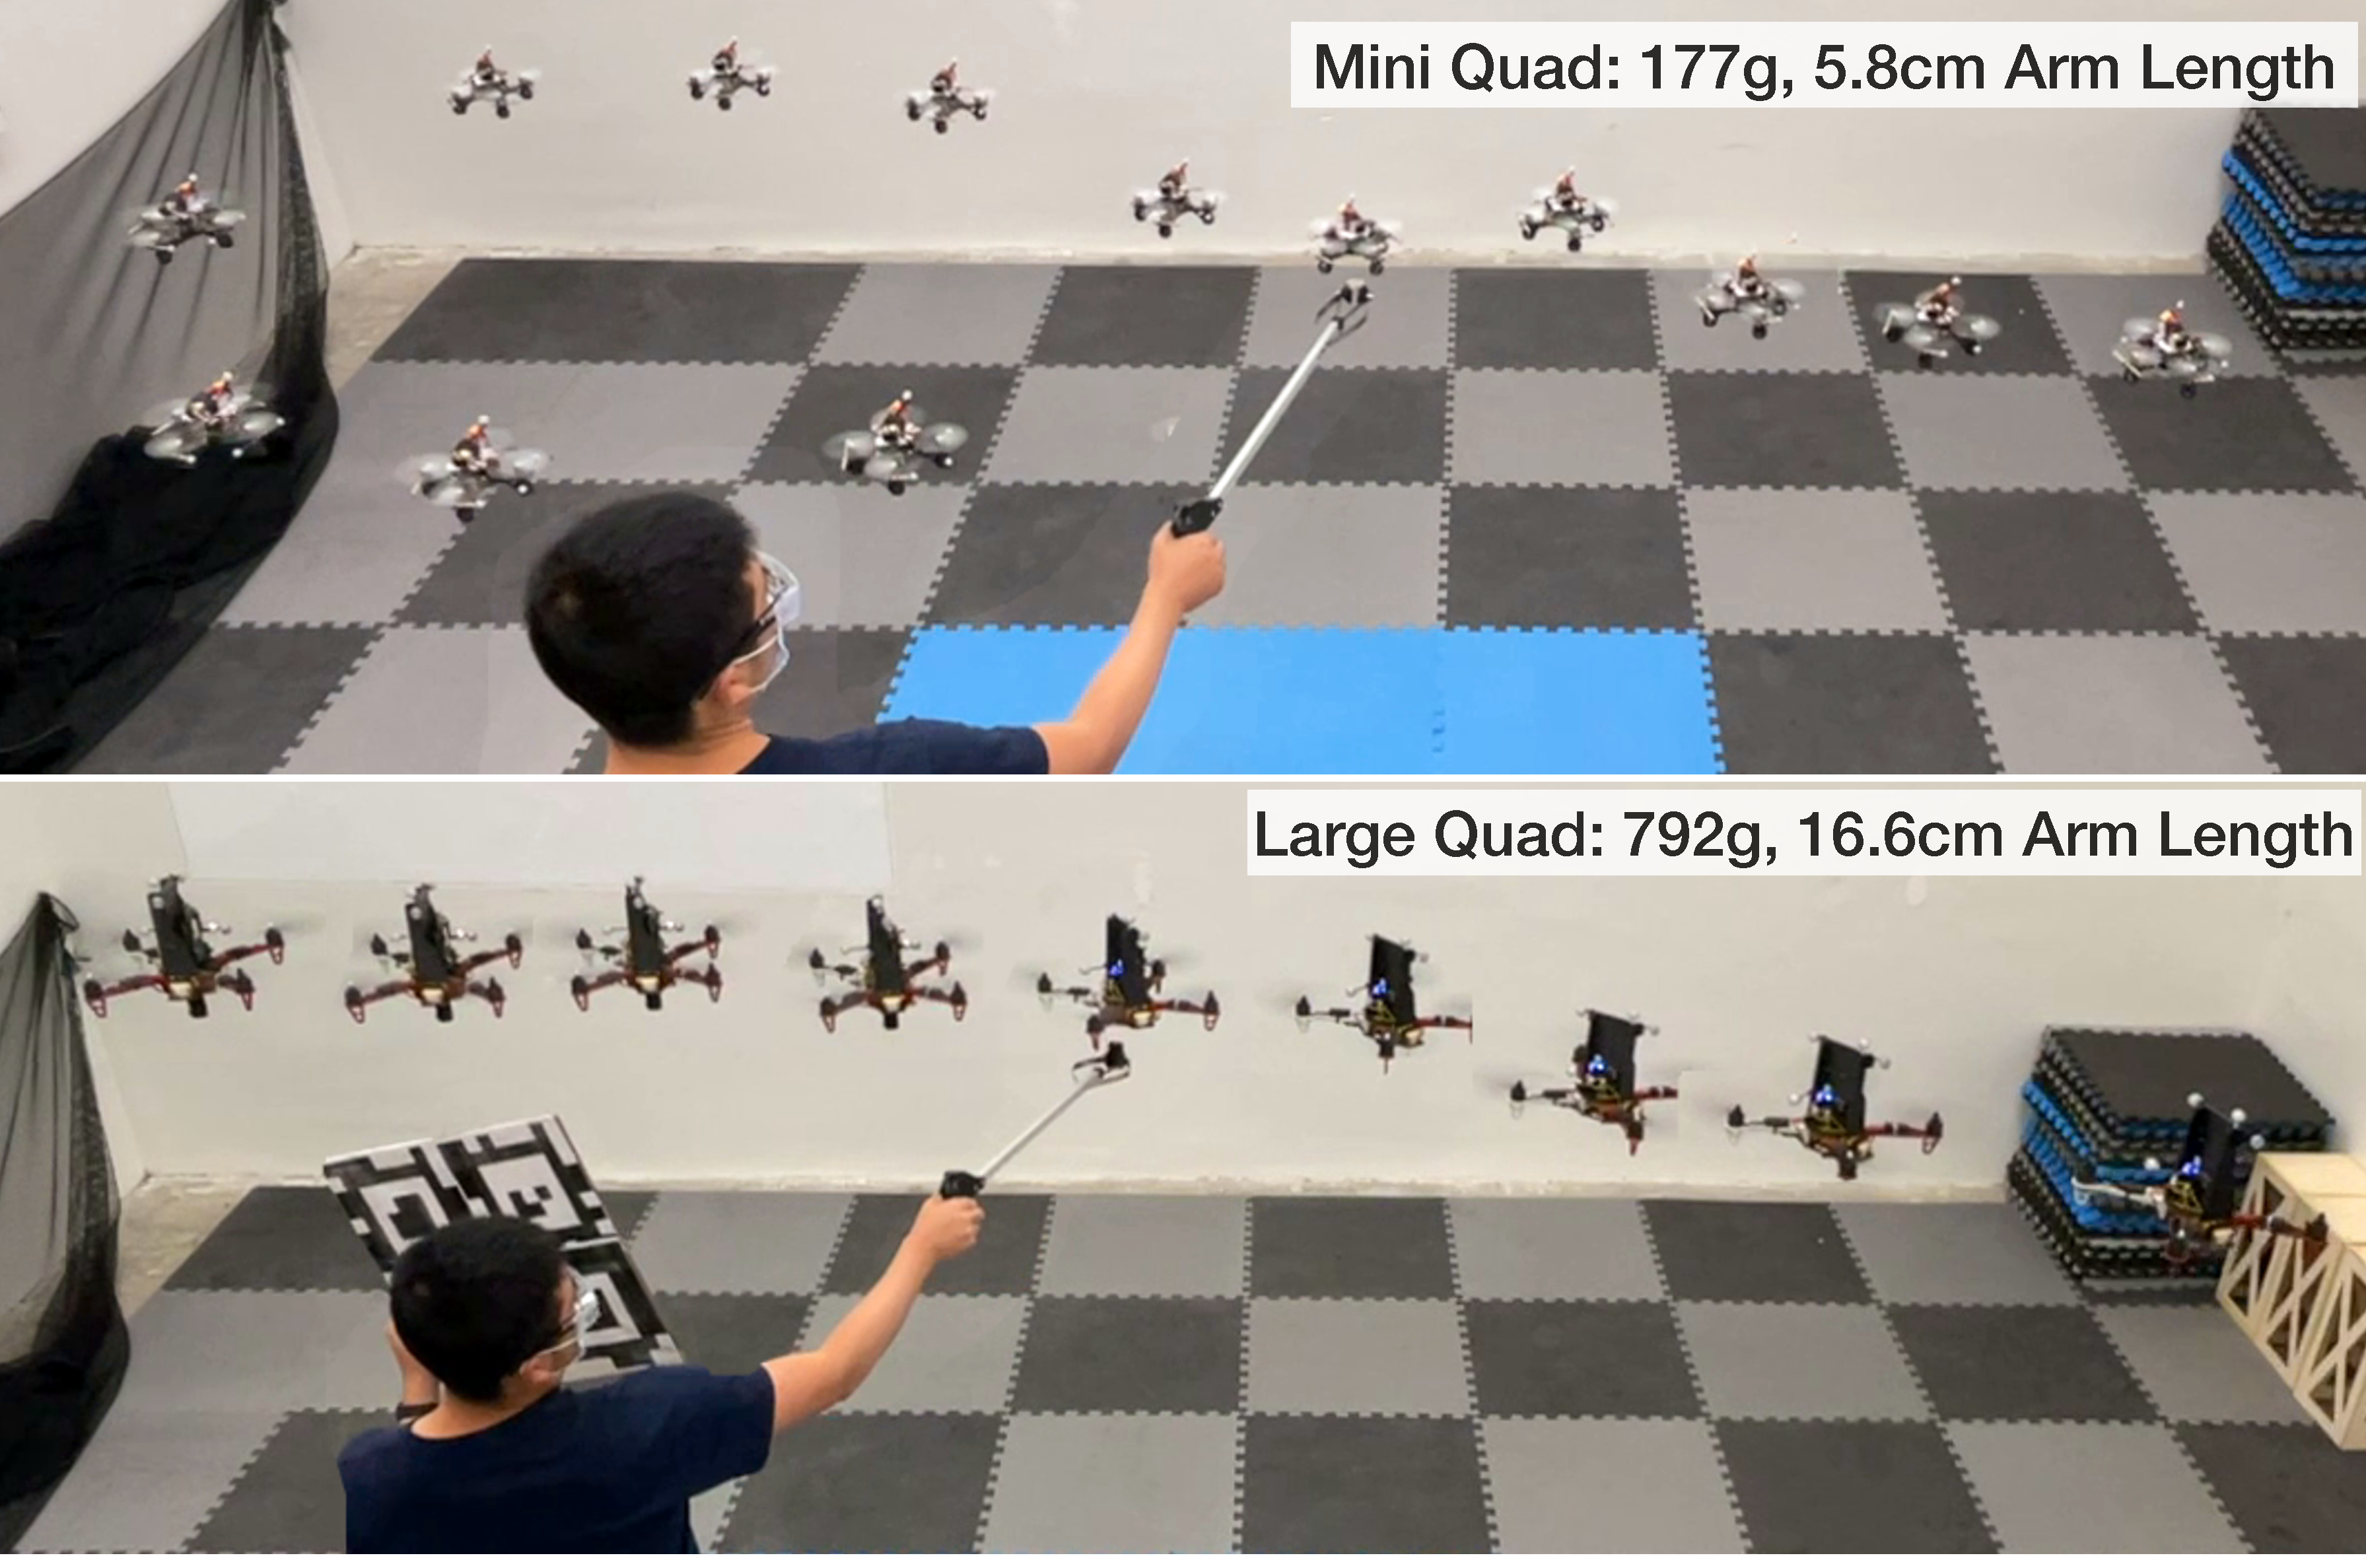
\includegraphics[width=\columnwidth]{img/figure1.pdf}
\captionof{figure}{\small Demonstration of our adaptive controller on two quadrotors with widely varying mass, arm length, and motor constants for the task of tracking a straight and circular trajectory. In the middle of the trajectory, we add a payload unknown to the drone of approximately 30\% of the robot's mass. Our end-to-end controller is able to quickly estimate and react to the disturbance. In both the demonstrations described above and all the simulation and real-world experiments presented here, we use a single control policy across different drones and tasks, which is deployed without any modifications or tuning.}
\label{fig:teaser}
\vspace{-3ex}
\end{figure}

% \todo{change the notation of low level controller}

% \propose{\begin{itemize}
%     \item in robotics field, we have good solutions in specific tasks. 
%     \item gives rise to an idea for general purpose solution 
%     \item we think this problem in quadcopter controller settings
%     \item quadcopters are good in easy access and wide range of application  
%     \item a good controller need knowledge of the model and careful tuning 
%     \item traditional (PID), RL, all control them well
%     \item However, they are platform-specific. often fails when transferring to new models. need start from scrach training for learning controller, or specific tuning for traditional 
%     \item In addition, disturbance rejection are usually applied on the specific model and on specific disturbance. (need reference)
%     \item rejection to different disturbance, requires extensive data collections and simulated models  
%     \item a universal controller applied to different quadcopters to save the labor intensive work. And on general disturbances rejection at the same time.
%     \item Our controller is able to adapt based not only on morphology, but also down to hardware characteristic (one level higher).
% \end{itemize}}
% 
% \propose{\begin{itemize}
%     \item Adaptive control is cool and works (ref)
%     \item However, under the hood, those methods assume access to the underlying model of the platform and hardware.
%     \item This assumption is justified in a industrial setting (where all drones are the same).
%     \item However, what happens if we lift such assumption?
%     \item Why is this question important? Example: hobby or research drones (cite the several flight stacks).
%     \item Doing so requires a "universal" controller, that can adapt not only to disturbances, but also to the morphology and hardware of the robot.
%     \item In this paper, we use a learning-based adaptive controller to solve this problem.
%     \item The controller is robust to unseen disturbances at train time.
%     \item This approach works better than existing methods.
%     \item We extensively test it in both sim and real world.
% \end{itemize}
%
%Adaptive control for aerial vehicles has been a top priority for research for decades. 
% %
% It has achieved great access in extensive scales of applications from an indoor quadcopter~\cite{hanover2021performance} to a civil transport aircraft~\cite{doi:10.2514/6.2009-5738}.
% %
% However, with its approaches greatly evolving, it assumes access to the underlying model of the platform and hardware.
% %
% Adaptive control is greatly concerned with estimating and conteracting disparities between observation and a \emph{reference} model. 
% %
% This assumption leads one to wonder: what happens if we can lift such assumption? 
% %
% If so, the controller can completely bypass the notion of a reference model, which enables adaptation not only to disturbances and model uncertainties, but also to the morphology and hardware of the robot. 
% %
% This much wider range of adaptation can greatly save the labor-intensive process of designing controllers for quadcopters.
% %
% % Recent years have witnessed the growing interest in quadcopters due to its versatility in applications.
% % %
% % Such growing interest has lead to the emergence of commercially available and customizable quadcopters for hobbyists and researchers. 
% %
% Designing optimal controllers for quadcopters is challenging, as it requires accurate knowledge of the dynamics of quadcopters and careful controller design for desired skills. (basically copied from locomotion paper)
% %
% Poorly designed controllers can lead to suboptimal performances for quadcopters. In some cases, they may even become potentially danguerous for quadcopters such highly dynamic systems, since failure to control quickly leads to a crash. 
% %
% Flight stacks like PX4~\cite{PX4} and Beta-Flight~\cite{BetaFlight} have enabled the design process easier, but they still requires significant in-flight tuning for each quadcopter type and are generally tailored to human pilots. 
% %
% %
% }

% \propose{
% \begin{enumerate}
%     \item Optimal control of quadcopter requires a delicate design of controller. 
%     \item This controller requires accurate model estimtion.
%     \item Laborious procedure description 
%     \item Laborious procedure will be eased if a single controller exists. 
%     \item Not existed, because it's hard with unstable dynamics.
%     \item Model uncertainty and disturbance rejection requires more layer of complexity
% \end{enumerate}
% }

% \todo{The joy of the design and assembly of a new quadcopter is generally followed by great despair.
% %
% Once the hardware is in place, getting the quadcopter into the air may apparently look like a simple task.
% %
% Well-established systems provide a simple way for generating trajectories and high-level controllers for tracking them (e.g., \cite{mueller2019trajectory,mellinger2012trajectory,kaufmann2020RSS}).
% %
% Such high-level controllers generally abstract action in terms of thrust and angular rates.
% %
% The interface between these actions and motor commands, physically executable by the hardware, is an \emph{appropriate} low-level controller. % that, e.g., meet certain specification on closed-loop time constants.
% %
% And here is where the headaches start.}

A classic controller for quadcopters requires explicit estimates of the vehicle's model, including inertia properties (MMOI and mass), motor constants, and other parameters.
%
Errors in estimating such parameters directly translate to errors in the execution of the controller commands.
%
In addition, once the parameters are estimated, the controller requires specific tuning in-flight to achieve the desired behaviour.
%
% If the estimation and tuning is done right, the final performance will be very good.
%
% But what looked like a simple task required significant engineering effort.
%
A small modification to the vehicle, e.g., replacing the motors with ones that have different properties or a different shape, would require repeating the above steps in estimation and tuning.
%
Such significant engineering efforts could be eased with a single controller without specialized tuning. However, this problem raises several challenges since quadcopters are very unstable systems. 
%
Large variations in quadcopter design have prompted the design of specialized controllers for different quadcopters, as opposed to one single controller. 
%
Rejection to disturbances or model uncertainties requires non-trivial design changes to the specialized controllers, which add more layers of complexity to the design work.
%
% Such engineering effort is compounded when the vehicle has variable properties, e.g., can carry different payloads or has a changing shape~\cite{falanga2018foldable,derrouaoui2022adaptive}.
% %
% Moreover, additional engineering effort and tuning is required if the controller needs to be robust against model uncertainties or external disturbances, e.g. aerodynamics effects or wind~\cite{shi2019neural, neuralfly, torrente2021data}.

% \todo{Introduction
% This section could be better organized to motivate why a
% universal controller is important, and why existing
% approaches do not serve as universal controllers. More
% specifically:
% Organization:
% Authors should provide motivation (e.g. autopilot without
% tuning) in the first paragraph before beginning a
% discussion on why the universal control problem is
% technically challenging.
% Authors should briefly state what their universal
% controller actually accomplishes (e.g. low-level control of
% thrust and angular velocity), which is not clear in the
% introduction.
% Discussion related to the technical challenge of the
% problem is scattered through the introduction and can be
% consolidated. 
% The reasoning behind why past approaches are not
% universal drone controllers should be better justified.}

% In this paper, we show the first universal controller for quadcopters. 
% %
% Quadcopters are inherently unstable and require high-frequency control of up to 500Hz. 
% %
% Failure to adapt to perturbations within fractions of a second can potentially lead to a crash.
% %
% Consequently, a universal controller should not only be able to handle diverse perturbations, it should do so very fast. 
%
% \todo{The introduction indicates that the controller is able to adapt to new situations within 0.8 sec (which corresponds to the window of 400 steps). But in Section V.C, empirical results indicate that the adaptation period is close to 2 secs.}
% 
In this work, we show the first controller aiming to control a variety of quadcopters with differences in mass, armlength, motor constant, etc. of up to 4 times within one second, without any modification or fine-tuning for the specific quadcopters. Our controller is a near-hover position controller capable of flying vastly different quadcopters to target positions.
%
In addition, our controller can rapidly adapt to unknown disturbances in the mass and inertia changes of the quadcopters.
%
Our work builds on three main insights.
%
The first is that the dynamics parameters are observable from the history of states and actions.
%
This has long been known in the community: several works have shown how to estimate parameters online with filters~\cite{svacha2020imu,wuest2019online} or with neural networks~\cite{forgione2021continuous}.
%
Yet, prior work overlooked the possibility of using these estimates to condition the controller's behaviour.
%
The second insight is that, at test time, we do not need an estimate of the parameters in some "ground truth" sense.
%
What matters is that the estimate leads to the "right" action, which our end-to-end training procedure optimizes.
%
This simplifies the estimation problem and avoids identifiability issues, e.g., identical effects on unobservable or unmatched uncertainties~\cite{hovakimyan2010l1}.
%
% The third and final insight is that a system trained to adapt to a large variety of morphological and dynamical parameters is automatically robust to disturbances which are very difficult to model and to train on, \emph{e.g}, aerodynamics effects or swinging payloads.
%
% \todo{When the authors enumerate the three insights leveraged by their algorithm, the third comment about the algorithm being robust to disturbances within the convex hull of the training should be substantiated. }
%
The third and final insight is that a system can adapt to previously unseen disturbances as long as their effect on the platform dynamics is in the convex hull of the training disturbances (e.g., a motor losing efficiency has a similar effect to adding a payload below the motor).
%Therefore, future work should not spend effort on simulating all possible disturbances but on finding the minimal set of parameter changes to trigger a reaction.}
% we can train both the controller and the latent parameter identification module in simulation, where both the ground truth values and the state-action history are available. \antonio{The last insight is a bit less "insightful" than the others, maybe remove?}

To operationalize this, we follow the approach initially proposed for legged robots~\cite{kumar2021rma}. However, while this work performs online adaptation to terrains, we use their approach to adapt to a diverse set of quadcopter bodies and perturbations. Specifically, we estimate a latent representation of the quadcopter's body from a history of sensor observations and actions, which conditions the behaviour of the controller.
%
%Such representation conditions the behaviour of the low-level controller.
The space of quadcopter properties in which we train is extremely diverse (Table~\ref{tab:randomization}).
%
%\antonio{The flow here is okaish, but don't know how to improve it}.
%
This diversity enables adaptation to sudden changes in environment conditions, e.g., a payload, for which it was not explicitly trained.
%
Our approach frees drone designers from the estimation and tuning process required any time something changes, or the risk that parameter changes unwittingly cause the control behaviour to significantly change, potentially endangering the system.
%
Furthermore, it naturally lends itself for use in off-the-shelf autopilot systems, allowing users who might otherwise lack the modelling abilities to control a custom vehicle, simply by plugging in the autopilot and not requiring any parameter tuning.

% \begin{itemize}
%     \item You get a new quadcopter.
%     \item You want it to perform a simple trajectory tracking task, and have access to any one of a number of well-established trajectory generation and high-level control (e.g., \cite{mueller2019trajectory}). These high-level controllers often treat as control input the vehicle angular velocity, which is assumed to be tracked by an appropriate low-level control that, e.g., meet certain specification on closed-loop time constants.  
%     \item Such low-level control requires estimates of vehicle inertia properties (MMOI and mass), motor constants, and other parameters; errors in estimating such parameters directly translate to errors in the low-level tracking performance. 
%     \item Once these are estimated, the controller is typically tuned in-flight to achieve the desired behaviour.
%     \item If you do all steps right, you get a good controller. But what was supposed to be a simple task required significant energy and engineering effort, and modifying the vehicle (e.g., by replacing the motors with ones that have different properties, and different mass) would require repeating the above steps.
%     Moreover, if the vehicle has variable properties (e.g., can carry different payloads) the effort is compounded.
% \end{itemize}


% \begin{itemize}
%     %\item In this paper, we propose a way to escape this important yet tedious step
%     %\item we propose a learning-based controller that can autonomously adapt to a new vehicle or to changing parameters
%     %\item To do so, our approach estimates a latent representation of the quadcopter's body from an history of sensor observations and actions.
%     %\item Such representation conditions the behaviour of the low-level controller.
%     %\item Not only can our approach quickly adapt to a new body, but also react to sudden changes in environmental conditions, e.g. wind, a payload, etc, for which it was not explicitly trained for.
%     % \item Such an approach potentially allows for a much larger exploration in the drone design, since designers do not have to repeat the estimation and tuning process any time something changes.
%     % Furthermore, the approach naturally lends itself for use in off-the-shelf autopilot systems, allowing users who might otherwise lack the modelling abilities to implement a low-level controller on a custom vehicle, simply by plugging in the autopilot and not requiring any parameter tuning. 
% \end{itemize}


%\begin{itemize}
    %\item The first insight behind our work is that the body parameters are observable from the state action history.
    %\item This has long been known in community, with several work showing how to estimate parameters online.
    %\item While this can be done with filters, or with NN. The first is provable under assumption, the second general works across a larger variety of dynamics.
    %\item NN are also especially good at estimating parameters and at working over across dynamics.
    %\item Yet, prior work overlooked the possibility of estimating those parameters \textbf{at test time} and use them to condition the low-level controller.
    %\item The second insight is that we do not need to explicitly estimate the parameters.
    %\item What we need is a low-dimensional projection of them which is relevant for control. 
    %\item If a change in payload or inertia exhibit the same form of disturbance to the quadcopter, they need to be projected to the same point in the manifold.
    %\item This largely simplifies the estimation effort at test time.
    %\item The third and final insight of our work is that we can try both the controller and the latent body identification module in simulation, where both the ground truth parameters and the state-action history are available.
%\end{itemize}

\begin{figure}
\centering
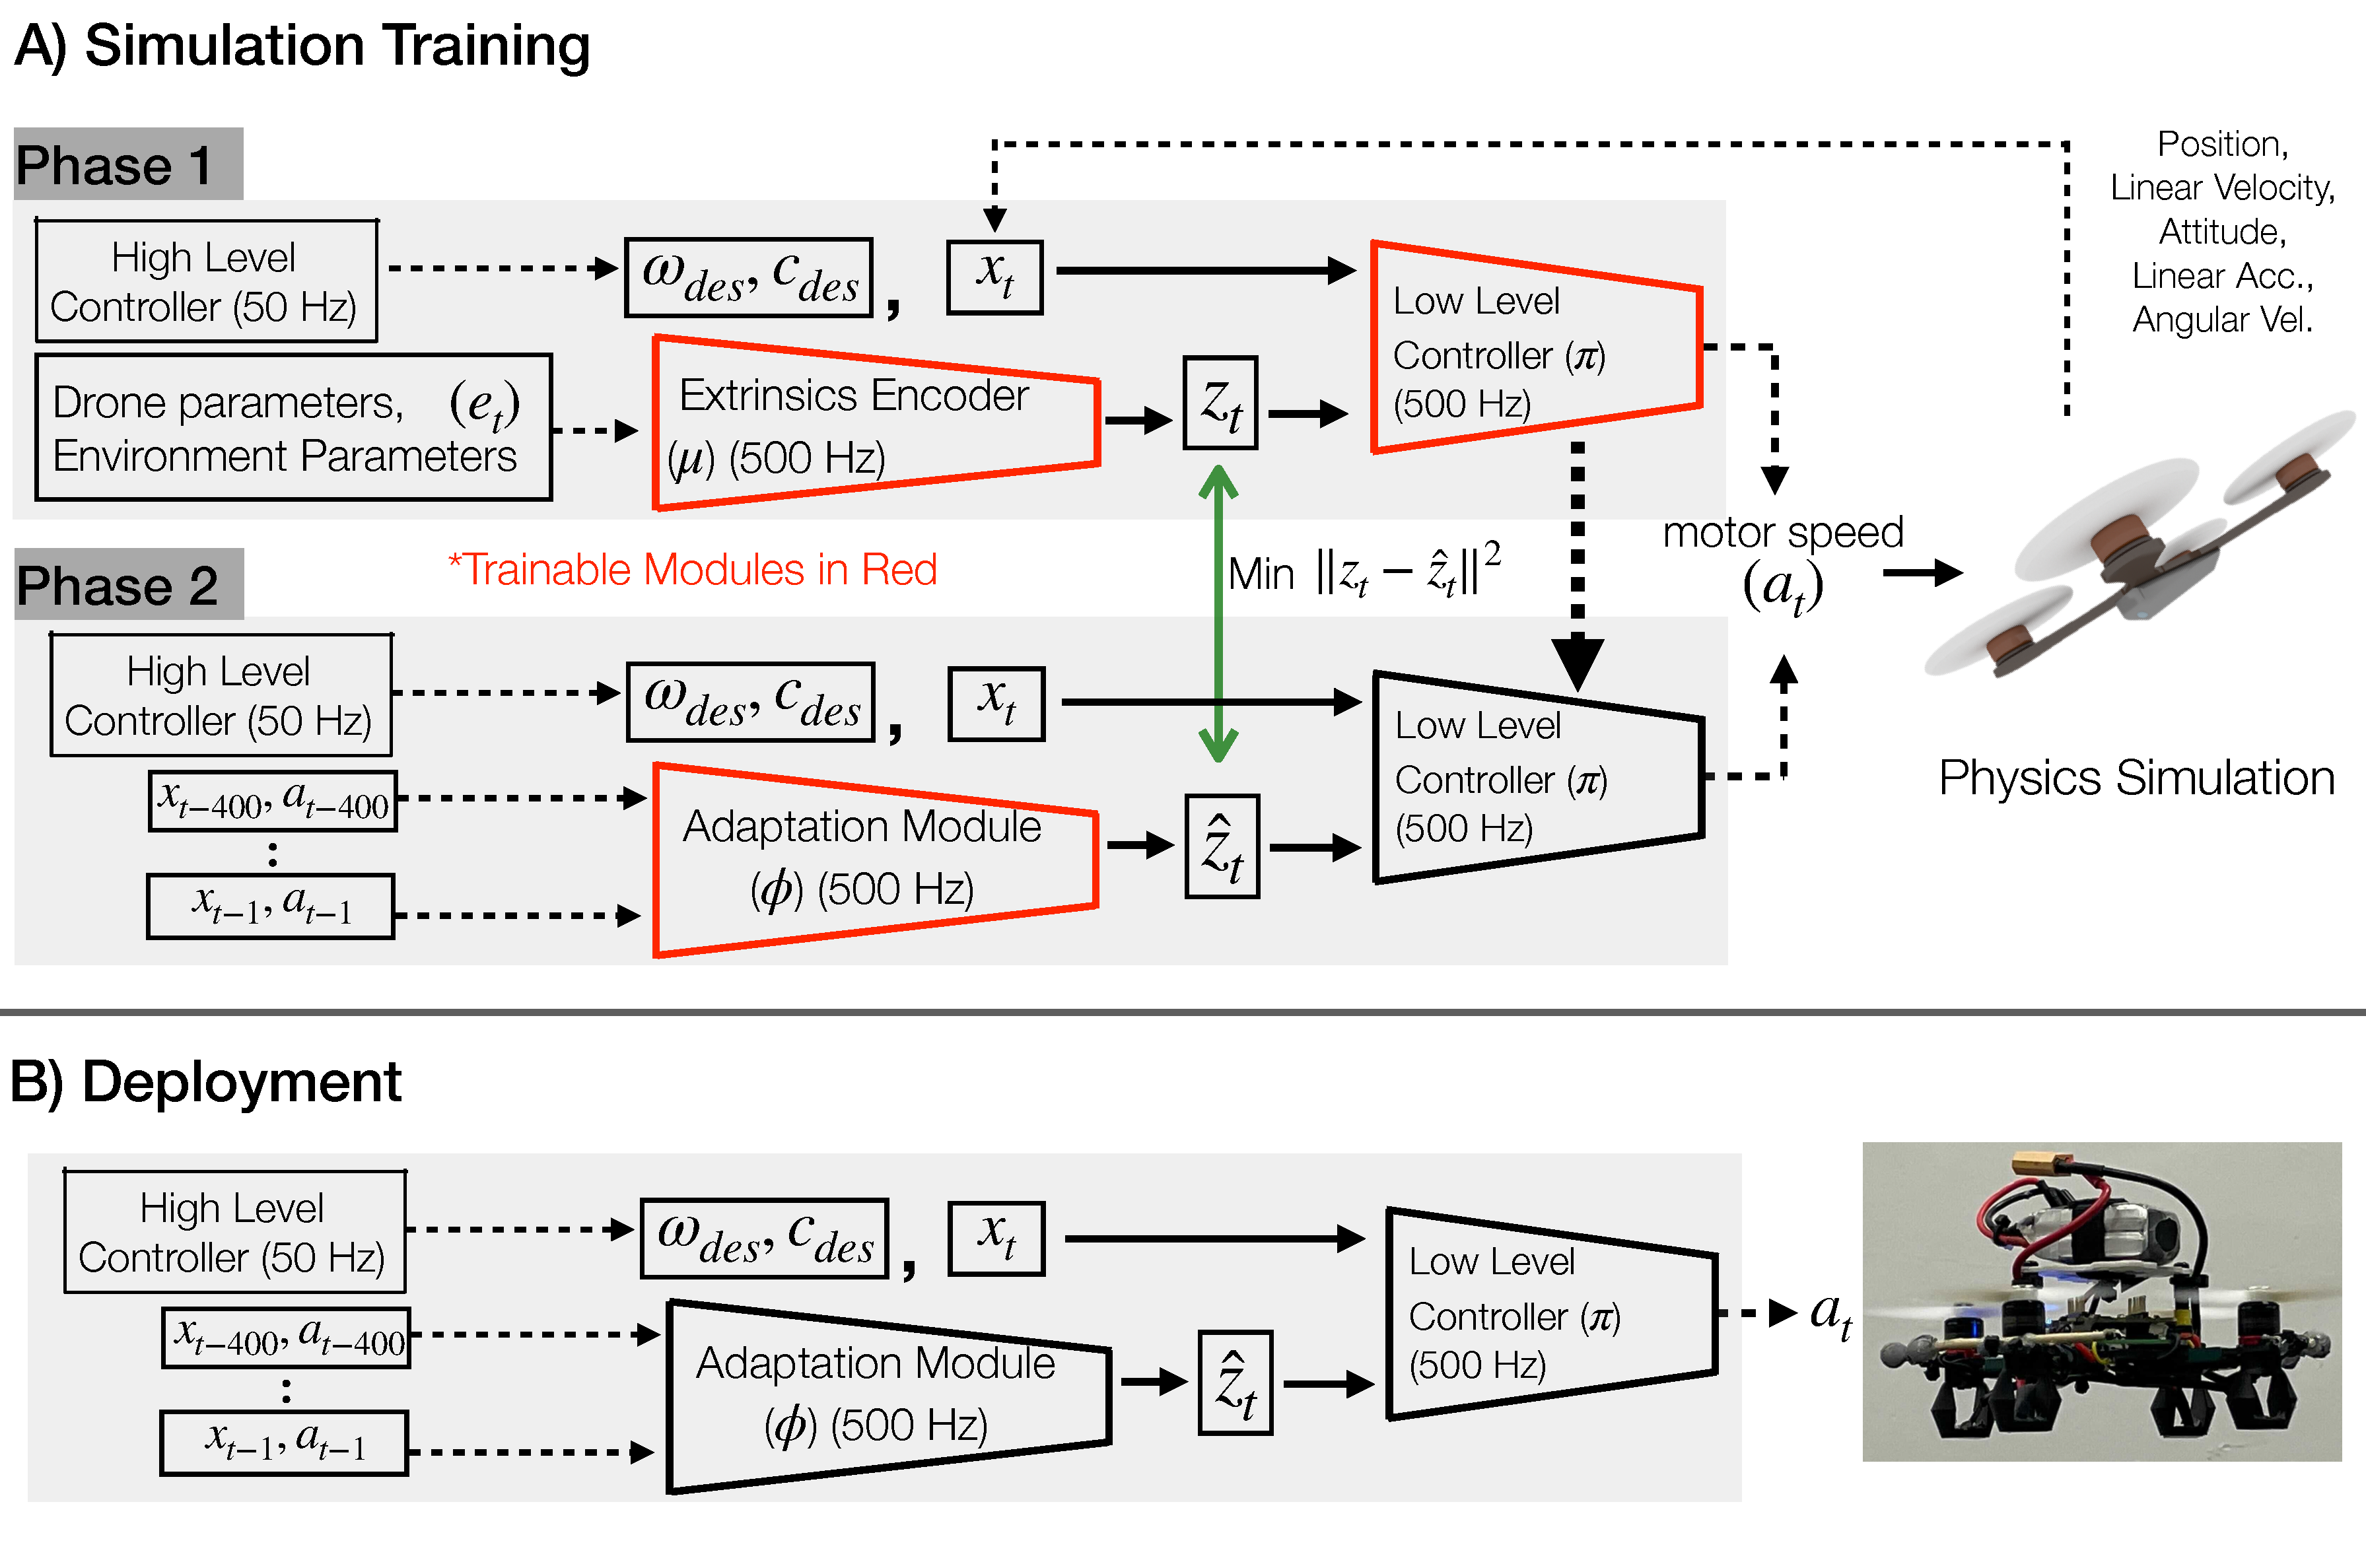
\includegraphics[width=\linewidth]{img/method-figures-no-last-act.pdf}
\caption{\small We show the training at the top and the deployment architecture of our system. We train in two phases. In the first phase, we train a base policy $\pi$ which takes the current state $x_t$, and the intrinsics vector $z_t$ which is a compressed version of the environment parameters $e_t$ generated by the module $\mu$. Since we cannot deploy this policy in the real world because we do not observe the environment parameters $e_t$, we learn an adaptation module which takes the sensor history and action history, and directly predicts the intrinsics vector $z_t$. This is done in phase two in simulation using supervised learning. We can finally deploy the base policy $\pi$ which takes as input the current state $x_t$ and the intrinsics vector $\hat{z_t}$ predicted by the adaptation module $\phi$.}
% \vspace{-5ex}
\label{fig:method}
\end{figure}

Our approach is related to existing methods in adaptive control.
%
However, our work shifts the meaning of adaptation to a different paradigm.
%
While adaptive control is generally concerned with estimating and counteracting disparities between observations and a \emph{reference} model, our approach does not have this notion. % of reference model.
%
This key difference enables adaptation to a much wider range of dynamics and disturbances.
%
In addition, it waives the engineering and tuning required by prior work when modifying the vehicle.
%
% Meta-learning is also related to the context of our problem in providing fast online adaptation.
% %
% Although they have been demonstrated on real quadcopters with impressive results on disturbance rejection~\cite{belkhale2021model,neuralfly}, they require real world learning samples to adapt.
% %
% When adapting to a much wider scale in our problem setting, this approach could be potentially dangerous for a dynamic system like a quadcopter, since failure to adapt quickly leads to catastrophic failure (a crash).
%
The closest related to our work are industrial systems like Beta-Flight~\cite{BetaFlight} and PX4~\cite{PX4}.
%
While they work well across a variety of vehicles, they still require significant in-flight tuning for each robot type and are generally tailored to human pilots.
%
% Finally, our work is also related to existing approaches in legged locomotion~\cite{kumar2021rma,lee2020learning}.
% %
% These works perform online adaptation to navigate a large variety of terrains.
% %
% However, while they adapt to different external factors (friction, terrain geometry, payload), they still rely on an accurate dynamic and morphological model of the platform \propose{to perform on one single robot}.
% %
% Therefore, changes to the robot would inevitably lead to re-training of the control policy. 
% \todo{Meta-RL}
% \propose{
% \begin{itemize}
%     \item Meta-RL is also related to our method. 
%     \item It gathers real world data to learn a latent representation of unknown disturbances or model uncertainties, then uses the learned latent to augment the base controller's performance during test time~\cite{belkhale2021model,neuralfly}
%     \item They still just perform on one platform. 
%     \item Their approach may be dangerous in our problem with the much wider range of dynamics and disturbances for dynamics systems as drones
%     \item However meta-learning could be used to complement our work in the future for a better performance 
% \end{itemize}
% }
% \begin{itemize}
%     \item Our approach is related to traditional adaptive control.
%     \item Adaptive control works well but still requires platform-specific design and tuning.
%     \item The closest related to our work are industrial systems like Beta-Flight or PX4.
%     \item They work well across vehicles, but they require tuning every time a vehicle changes.
%     \item They are also designed to work well for human pilots flight.
%     \item Our work is also related to existing approaches in legged robotics
%     \item There similar insights to ours have been used to unlock locomotion on a different set of terrains in a seamless fashion.
%     \item However, they show adaptation to different external factors (friction, terrain geometry, payload), but not to the robot body itself.
%     \item Indeed, they rely on a quite accurate system of the platform in term of platform geometry and actuation.
%     \item Some of them even rely on special purpose motor models which can only be trained with more than 30min of experience on the physical robot, and would need to be retrained any time the physical robot changes.
% \end{itemize}

% \subsection{Contributions}

% \antonio{Not really a fan of this section, would prefer to remove it}.
% We present the first universal low-level controller for quadcopters.
% %
% Our controller can cope with large variations in actuation and dynamics of the platform~\todo{quantify}.
% %
% In addition, it can react to disturbances which are difficult to model, \emph{e.g.} aerodynamics, and for which it was not explicitely trained for.
% %
% We compare our approach against baselines both in simulation and in the physical world and obtain results of up to X\% better in terms \todo{finish when we know the results}.
% %
% This work allows minimising the engineering effort required when building new platforms, potentially opening the door of drone design to a much larger audience than was previously possible.


% \begin{itemize}

%     \item We present the first universal low-level for quadcopters
%     \item It can cope with large variations in actuation and dynamics of the platform (up to 2 orders of magnitude
%     \item We compare our approach against baselines both in simulation and in the physical world and obtain results of up to X\% better in terms \todo{finish when we know the results}
%     \item This work allows to minimize the engineering effort required when building new platforms.
%     \item Easing the control problems, it potentially opens the door to a much wider space of designs and enlarges the set of people who can build drones.
    
% \end{itemize}


% \emph{What is the problem? Why is it important?}

% \emph{Why is the problem hard? What makes it challenging?}

% \emph{How far has existing work come? Why hasn't the problem been solved? What is the stumbling block? What is the frontier?}

% \emph{What does our paper contribute? What is the key idea? What is the magic trick? What is the new insight or technique that enables us to advance the frontier?}

% \emph{Any other interesting aspects of the approach or its execution?}

% \todo{Want to make sure that we emphasize that model-based control gives us very strong performance. However, creating the control requires knowledge of system parameters, like inertial parameters, motor characteristics, etc. Thus, when implementing a model-based control on a new drone, the engineer typically has to spend significant energy on estimating parameters, and tuning constants, to get the desired behaviour. Having a system that can quickly adapt to a new vehicle, and keep adapting as the vehicle's payload and environmental conditions change, would make it much easier to control a variety of vehicles with minimum engineering effort.}